\documentclass[12pt]{article}


\usepackage[
	a4paper, 
	margin=2.5cm]{geometry}
\usepackage[utf8]{inputenc}         % UTF8 enkodiranje
\usepackage[slovene]{babel}          % Slovenščina
\usepackage[
	pdfusetitle, 
	hidelinks, 
	unicode]{hyperref}              % Nastavi atribute PDF-ja, ne označuj povezav
\usepackage{microtype}              % Izboljšave za tipografijsko perfekcijo :)
\usepackage{enumitem}               % Seznami za člene
\usepackage{graphicx}               % Vključitev slik
\usepackage{dirtytalk}              % Citat
\usepackage{listings}               % Kodni blok
\usepackage{fancyvrb}
\usepackage[font=]{caption}         % Required for specifying captions
\usepackage[normalem]{ulem}         % Krašanje enot v enačbi
\usepackage{times}                  % Times New Roman pisava
\usepackage{tikz} 
\usetikzlibrary{patterns}
\usetikzlibrary{arrows}
\usetikzlibrary{decorations.pathmorphing,patterns}
\usepackage[european]{circuitikz}   % Električna vezja
\usepackage{datetime}               % Datum
% \usepackage[slovenian]{csquotes}
\usepackage{braket}
\usepackage{amsmath} % matematika ki izgleda lepo
\usepackage{amsfonts} % množice
\usepackage[style=ieee, maxbibnames=3, minbibnames=1, 
maxcitenames=1, mincitenames=1, sorting=nyt]{biblatex}   % Navajanje virov
\bibliography{viri}

\urlstyle{rm}

\setlength{\parindent}{0em}
\setlength{\parskip}{1ex}

\setcounter{secnumdepth}{5}
\setcounter{tocdepth}{4}

\renewcommand{\thesection}{\arabic{section}}
\renewcommand{\thesubsection}{\thesection.\arabic{subsection}}
\renewcommand{\thesubsubsection}{\thesubsection.\arabic{subsubsection}}
\renewcommand{\theparagraph}{\thesubsubsection.\arabic{paragraph}}
\renewcommand{\thesubparagraph}{\theparagraph.\arabic{subparagraph}}

\renewcommand{\labelnamepunct}{\addcomma\space}
\DeclareFieldFormat[article]{title}{#1}
\DeclareFieldFormat[online]{title}{\mkbibemph{#1}}

\DefineBibliographyStrings{slovene}{
	andothers = {et. al\adddot},
	urlseen = {dostopano:}
}
	% Adapted from the 'patterns' library: enlarged the distance between the lines from 4pt to 10pt
\pgfdeclarepatternformonly{north east lines wide}{\pgfqpoint{-1pt}{-1pt}}{\pgfqpoint{10pt}{10pt}}{\pgfqpoint{9pt}{9pt}}%
{
	\pgfsetlinewidth{0.4pt}
	\pgfpathmoveto{\pgfqpoint{0pt}{0pt}}
	\pgfpathlineto{\pgfqpoint{9.1pt}{9.1pt}}
	\pgfusepath{stroke}
}


\tikzset{%
	body/.style={inner sep=0pt,outer sep=0pt,shape=rectangle,draw,thick,pattern=north east lines wide},
	dimen/.style={<->,>=latex,thin,every rectangle node/.style={fill=white,midway,font=\sffamily}},
	symmetry/.style={dashed,thin},
}
	
\newdateformat{MMYYYYdate}{\monthname[\THEMONTH] \THEYEAR}

\title{Poročila maturitetnih vaj pri predmetu fizika}
\author{Jaka Kovač, G 4. b}

\begin{document}
\pagenumbering{arabic}

\begin{center}
	\thispagestyle{empty}
	\includegraphics[scale=1]{slike/logotip_vegova_leze_brezokvirja.png}
	\\
	\textbf{Vegova ulica 4, 1000 Ljubljana}

	\vspace{\fill} 
	Poročila vaj pri predmetu fizika

	\Huge{\textbf{Poročila maturitetnih vaj}}

	\normalsize
	\vspace{\fill}

	Mentor: Tomo Omahna, prof. \hfill Avtor: Jaka Kovač, G 4. b\\
	\null
	Ljubljana, oktober 2023 – \MMYYYYdate\today %zamenjaj <mesec in leto> z mesecem in letom začetka
\end{center}
\newpage
\thispagestyle{empty}
\null
\newpage

\section*{Povzetek}
V tem delu bom predstavil kako sem izvedel maturitene vaje, njihove rezultate. Ob vsaki vaji
sem preverjal veljavnost meritev s teoretično izračunaimi vrednostmi.
\\ %prazna vrstica
\textbf{Ključe besede:} poročila maturitetnih vaj - fizika, fizika za srednjo šolo

\vfill

% KAZALO 
\newpage
\thispagestyle{empty} % ne številčimo strani
\tableofcontents % kazalo

\begingroup     % kazalo slik
\makeatletter
\section*{Slike}
\@starttoc{lof}
\let\clearpage\relax
\makeatother
\endgroup


\newpage

\section*{O zapisu meritev}
Prikazane številčne vrednosti so zaokrožene na 3 od 0 različna decimalna mesta (znanstven zapis).
V izračunih se uporablja dejanska vrednost. Kjer ni drugače navedeno je vrednost podana na
$\pm 0,5$ enot na zadnjem prikazanem mestu. Primer: $s = 10,0 \text{ m} = 10,0 \text{ m} \pm 0,05 \text{ m}$

\section{Lastno nihanje vzmetnega nihala}  --- NOT DONE
	\subsection*{Opis vaje in teoritična podlaga}
	Nihanje količine $x$ lahko zapišemo z enačbo nihanja
	\begin{equation}
		\frac{d^2 x}{dt^2} + \omega_0^2 x = 0 .
	\end{equation}

 

	V našem primeru želimo preveriti sinusno nihanje vzmetnega nihala.
	Hookov zakon pravi, da je $F_v = -ks$, po II. Newtonovem zakonu pa lahko zapišemo 
	\begin{equation}
		F_v = ma = -ks = m \frac{d^2 x}{dt^2} .
	\end{equation}
	Rešitev dane diferencialne enačbe je
	\begin{equation}
		x(t) = x_{max} \sin(\omega t + \varphi); \omega = \sqrt{\frac k m} \land \varphi = \arcsin(\frac{x(0)}{x_{max}}).
	\end{equation}
	\newpage
	
	

	\subsection*{Uporabljeni pripomočki}
	\subsection*{Grafi, ipd.}
	\subsection*{Analiza rezultatov}

\newpage
\section{Prosti pad}
 	\subsection*{Opis vaje in teoritična podlaga}
	Na Zemlji vsa telesa v prostem padu pospešujejo z $ a = g \approx 10 \frac{\text{m}}{{\text{s}}^2}$.
	Ta pospešek lahko izračunamo iz splošnega gravitacijskega zakona:
	\begin{equation}
		\label{gravity}
		\begin{split}
			F &= G \frac{mM}{r^2}; G = 6,67408 \pm 0,00031 \cdot 10^{-11} \frac{\text{N}\text{m}^2}{\text{kg}^2} \\
			a m &= G \frac{mM}{r^2} \\
			g &= G \frac{M_{Zemlje}}{{r_{Zemlje}}^2} \\
			g &\approx 6,67408 (1 \pm 4,64 \cdot 10^{-5}) \cdot 10^{-11} \frac{\text{N}\text{m}^2}{\text{kg}^2} \cdot \frac{5,972168 (1 \pm 8,37 \cdot 10 ^{-8}) \cdot 10^{24} \text{kg} }{(6,3710 (1 \pm 7,68 \cdot 10^{-6}) \cdot 10^6 \text{m}) ^2} \\
			g &\approx 9,826 (1 \pm 6,18 \cdot 10^{-5}) \frac{\text{m}}{\text{s}^2} \approx (9,826 \pm 0,000608) \frac{\text{m}}{\text{s}^2} \qquad \mbox{\cite{earth}}
		\end{split}
	\end{equation}
	Vrednost pa lahko imerimo tudi eksperimentalno. S senzorjem \footnote{fotovrata} lahko
	izmerimo prepotovano pot (prosto) padajočega telesa iz česa pa lahko izračunamo hitrost
	telesa in njegov pospešek.
	\begin{equation}
		\begin{split}
			s(t) &- \text{pot v odvisnosti od časa} \\
			v(t) &= \frac{ds}{dt} \\
			a(t) &= \frac{dv}{dt} = \frac{d^2s}{{dt}^2}
		\end{split}	
	\end{equation}


 	\subsection*{Uporabljeni pripomočki}
	Verinier-jev vmesnik, fotovrata, merilna letev z razmakom 1 cm med oznakami
	\vspace{\fill}

 	\subsection*{Grafi in izpis vrednost}

	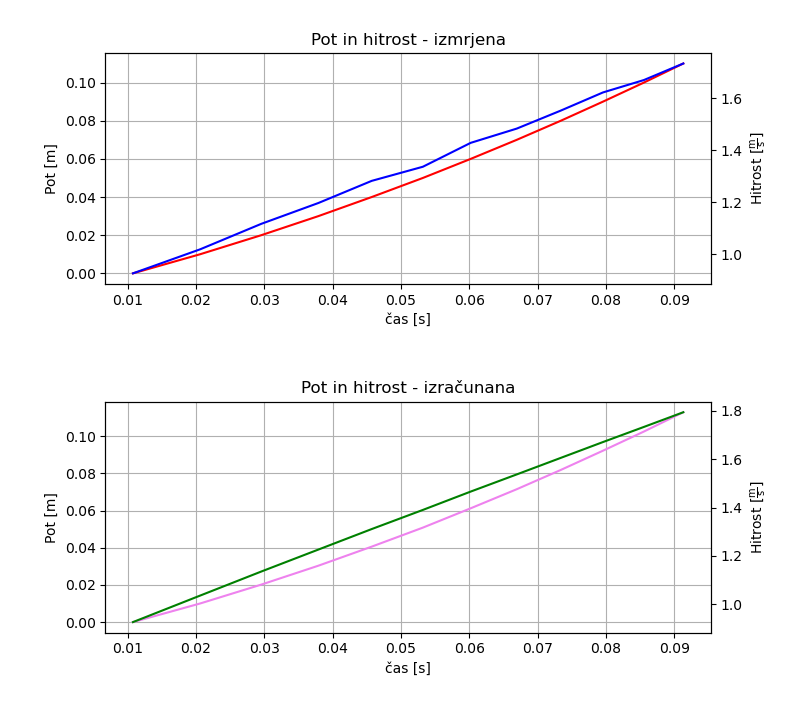
\includegraphics[width=\linewidth]{slike/graf_v2_1.png}

	\begin{table}[h!]
		\centering
		\begin{tabular}{|l|l|l|l|l|l|}
		\hline
		$t$ [s] 	& $s$ [m] 	& $v$ [$\frac{\text{m}}{\text{s}}$] & $a$ [$\frac{\text{m}}{\text{s}^2}$] 	& $s_i$ [m] 	& $v_i$ [$\frac{\text{m}}{\text{s}}$] 	\\ \hline
		0,010797	& 0			& 0,92618320						&  9,40661859							& 0				& 0,92618320							\\ \hline
		0,020615	& 0,01		& 1,01853738						& 10,96116178							& 0,01000000	& 1,03578499							\\ \hline
		0,02957		& 0,02		& 1,11669458						&  9,59826534							& 0,02016934	& 1,13544882							\\ \hline
		0,037925	& 0,03		& 1,19688809						& 10,91835783							& 0,03033728	& 1,22635222							\\ \hline
		0,045725	& 0,04		& 1,28205128						&  7,25793658							& 0,04058345	& 1,31116494							\\ \hline
		0,053208	& 0,05		& 1,33636242						& 13,14168756							& 0,05081054	& 1,39034378							\\ \hline
		0,060209	& 0,06		& 1,42836738						&  8,13883399							& 0,06121448	& 1,46630471							\\ \hline
		0,066951	& 0,07		& 1,48323939						& 10,76145884							& 0,07148008	& 1,53737279							\\ \hline
		0,073392	& 0,08		& 1,55255395						& 11,31882147							& 0,08184505	& 1,60581174							\\ \hline
		0,079556	& 0,09		& 1,62232317						&  7,96317857							& 0,09218808	& 1,67119519							\\ \hline
		0,085544	& 0,10		& 1,67000668						& 11,04308426							& 0,10248933	& 1,73376677							\\ \hline
		0,091312	& 0,11		& 1,73370319						& 11,30419690							& 0,11287113	& 1,79455176							\\ \hline
		\end{tabular}
	\end{table}

	Povprečni izmerjen pospešek je $\overline{a} = (10,3 \pm 2,2) \frac{\text{m}}{\text{s}^2} = 10,3 (1 \pm 0,21) \frac{\text{m}}{\text{s}^2}$, kar
	sem tudi uporabil pri izračunanih vrednostih poti in hitrosti.
 	\subsection*{Analiza rezultatov}
	Izmerjena vrednost je za okoli 5 \% večja od vrednosti izračunane v enačbi \eqref{gravity}.
	Ugotovil sem, da je napaka meritev tako velika, da je dejanksa vrednost znotraj merske
	napake. Do tako velike napake je verjetno prišlo, saj se je letev med padcem 
	\footnote{spust - ang. "descend"; padec - ang."fall" \cite{fallvsdescent}}
	premikala tudi bočno, s tem pa prepotovala daljšo pot, kot če bi padala navpišno navzdol.

\newpage
\section{Odbojnost}
	\subsection*{Opis vaje in teoritična podlaga}
	Meritev koeficienta odbojnosti albeda $a$ za različno obarvane podlage. Ker za referenco
	vzamemo bel papir, koeficient $a$ izračunamo po formuli:

	\begin{equation}
		a = \frac{E(obarvan \quad papir)}{E(bel \quad papir)},
	\end{equation}
	kjer $E$ predstavlja osvetljenost oz. površinsko gostoto svetlobnega toka. 
	\subsection*{Uporabljeni pripomočki}
	Mobilni telefon z aplikacijo za meritev osvetljenosti, namizno svetilko, bel in barven
	papir

	\subsection*{Meritve}
	\begin{table}[!h]
		\centering
		\begin{tabular}{|c|c|c|c|c|c|}
		\hline
		Barva papirja & $E_1$ [lux] & $E_2$ [lux] 	& $E_3$ [lux] 	& $\overline{E}$ [lux] 	& $a$   \\ \hline
		bela          & 331			& 332			& 334			& 332 					& 1     \\ \hline
		zelena        & 320 		& 322 			& 322 			& 321 					& 0,967 \\ \hline
		rdeča         & 314 		& 315 			& 315 			& 315 					& 0,949 \\ \hline
		oranžna       & 307 		& 308 			& 308 			& 308 					& 0,928 \\ \hline
		modra         & 299 		& 301 			& 300 			& 300 					& 0,904 \\ \hline
		rumena        & 326 		& 327 			& 327 			& 327 					& 0,985 \\ \hline
		temno modra   & 285 		& 285 			& 285 			& 285 					& 0,858 \\ \hline
		\end{tabular}
	\end{table}

	\subsection*{Analiza rezultatov}
	Vidimo, da ima "temnejši" papir manjši albeda faktor. Meritev bi lahko izboljšali, če 
	bi za osnovo uporabili ALU-folijo ali kaj podobnega. Bel papir zaradi površinske 
	hrapavosti svetlobo razprši, kar povzroči zmanjšanje izmerjene osvetlitve.

\newpage
\section{Boylov zakon}
	\subsection*{Opis vaje in teoritična podlaga}
	Za idealni plin velja splošna plinska enačba:
	\begin{equation}
		PV = nRT,
	\end{equation}
	kjer je $P$ tlak plina, $V$ njegov volumen, $n = \frac{m}{M}$ količina snovi (v molih),
	$R = 8,314 \frac{\text{m}^3 \cdot \text{Pa}}{\text{mol} \cdot \text{K}}$.
	\footnote{Plinska konstanta $R$ je definirana kot produkt Avogadrovega števila $N_A$ 
	in Boltzmanove konstante $k_B$. Vrednosti obeh sta bili z letom 2019 točno določeni, zato
	lahko izračunamo tudi točno vrednost $R$ \cite{redef}} Ko enačbo preuredimo, in upoštevamo, da količine
	plina v zaprtem postoru ne speminjamo (ohrani se $n$), lahko zapišemo:
	\begin{equation}
			\frac{PV}{T} = konst.
	\end{equation}
	Če plin ohranja temperaturo (sprememba je izotermna) dobimo Boylov zakon.
	\begin{equation}
		P_1 V_1 = P_2 V_2
		\label{boyle}
	\end{equation}

	\subsection*{Uporabljeni pripomočki}
	Brizga, Verinierjev vmesnik in senzor tlaka
	\subsection*{Grafi, ipd.}
	\subsection*{Analiza rezultatov}

\newpage
\section{Atwoodovo padalo}
	\subsection*{Opis vaje in teoritična podlaga}
	Atwoodovo padalo je George Atwood izumil kot enega izmed eksperimentlnih dokazov za
	Newtonov II. zakon. \newline
	
	Predpostavimo sistem mas, med seboj povezani z lahko vrvico, položene na lahek škripec.
	Ob začetku poskusa je sistem v ravnovesju, saj je na vsako stran vrvice obešena enaka
	masa $m_0 = 50,9$ g. Ko v sistem na eno stran dodamo $m_N = 54,9$ g, začne ta stran pospeševati
	proti tlom. 
	\begin{figure}[h!]
		\centering
		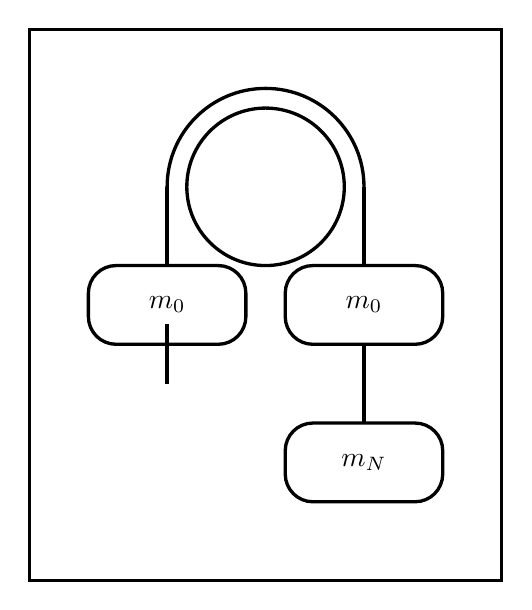
\begin{tikzpicture}
			\draw[black, very thick] (-3,-3.5) rectangle (3,3.5);
			\draw[black, very thick] (0, 1.5) circle (1cm);
			\draw[black, very thick] (1.25, 1.5) arc (0:180:1.25cm);
			
			%VRVICE
			\draw[black, very thick] (1.25, 1.5) -- (1.25, -1.5); %desna vrvica
			\draw[black, very thick] (-1.25, 1.5) -- (-1.25, 0.5); %leva vrvica
			
			%UTEŽI
			\draw[black, very thick, rounded corners=10pt] (-2.25, 0.5) rectangle (-0.25, -0.5) node (A) at (-1.25, 0) {$m_0$}; %leva m_0
			\draw[black, very thick, rounded corners=10pt, fill=white] (0.25, 0.5) rectangle (2.25, -0.5) node at (1.25, 0) {$m_0$}; %desna m_0
			
			\draw[black, very thick, rounded corners=10pt, fill=white] (0.25, -1.5) rectangle (2.25, -2.5) node at (1.25, -2) {$m_N$}; %desna m_N
	
			%SILE
			\draw[black, very thick] (A) -- (-1.25, -1);
			
			\end{tikzpicture}
		\caption{Atwoodovo padalo}
	\end{figure}

	Zapišemo lahko:
	\begin{equation}
		\begin{split}
			m_N \cdot g &= (2m_0 + m_N) \cdot a \\
			a &= g \cdot \frac{m_N}{2m_0 + m_N}
		\end{split}
	\end{equation}
	
	\subsection*{Uporabljeni pripomočki}
	različne uteži, sponke za papir, Verinierjev vmesnik, fotovrata s škripcem
	\subsection*{Grafi}
	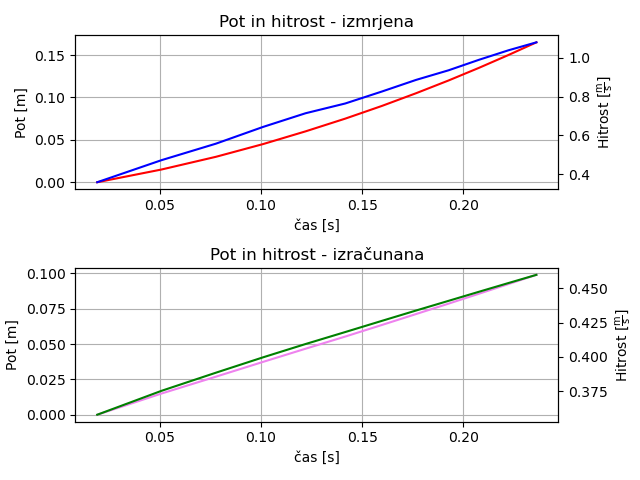
\includegraphics[width=\linewidth]{slike/graf_v5_1.png}

	\subsection*{Analiza rezultatov}
	Izmerjen pospešek je $a = 3,27 \pm 0.67 \quad \frac{\text{m}}{\text{s}^2} = 3,27 (1 \pm 0.21)\quad \frac{\text{m}}{\text{s}^2}$.
	Izračunana vrednost je $ a = 3,44 \quad \frac{\text{m}}{\text{s}^2}$ ker je znotraj 
	merske napake.

\newpage
\section{Dušeno nihanje v električnem krogu}
	\subsection*{Opis vaje in teoritična podlaga}
	Cilj vaje je izračunati koeficient dušenja $\beta$ v dušemen električnem nihajenm krogu.
	Začnimo z enačbo dušenega nihanja \cite{nihanje}
	\begin{equation}
		\frac{d^2 x}{dt^2} + 2\beta\frac{dx}{dt} + \omega_0^2 x =0 .
	\end{equation}
	V danem nihanjem krogu lahko z II. Kirchoffovim zakonom zapišemo
	\begin{equation}
		U - L\frac{dI}{dt} - RI = 0.
		\label{kirchoff}
	\end{equation}
	Tok v vezju lahko izračunamo z 
	\begin{equation}
		I = -\frac{de}{dt} = -\frac{d(CU)}{dt} = -C \frac{dU}{dt},
	\end{equation} ko tok vstavimo v enačbo \ref{kirchoff} dobimo
	\begin{equation}
		\begin{split}
			U + LC \frac{d^2U}{dt^2} + RC \frac{dU}{dt} = 0 \\
			LC \frac{d^2U}{dt^2} + RC \frac{dU}{dt} + U = 0,
		\end{split}
	\end{equation} če enačbo delimo z $LC$ pri tem pa upoštevamo $LC = \frac{1}{\omega_0^2}$ 
	lahko zapišemo
	\begin{equation}
		\frac{d^2U}{dt^2} + \frac{R}{L} \frac{dU}{dt} + \omega_0^2U = 0
	\end{equation} iz česar sledi, da je $x = U$ in $2\beta = \frac{R}{L}$ v enačbi dušenega
	nihanja. 
	Zapišemo lahko \cite{vaje}
	\begin{equation}
		U = e^{-\beta t}[A \sin(\omega t) + B \cos(\omega t)]
	\end{equation} kjer je $\omega = \sqrt[2]{\omega_0^2  - \beta^2}$ in $\beta = \frac{R}{2L}$.
	Ker poznamo začetne pogoje $(\frac{dU}{dt})_0 = - \frac{I_0}{C}$ in $U_0 = I_0 R$ lahko
	zapišemo končno enačbo za napetost
	\begin{equation}
		U = U_0 \cdot e^{-\beta t} \sin(\omega t).
	\end{equation}
	\subsection*{Uporabljeni pripomočki}
	Digitalni osciloskop, nihajni krog z elektrosnikim stikalom, ŠMI z žicami

	\newpage
	\subsection*{Posnetek zaslona osciloskopa}
	\begin{figure}[h!]
		\centering
		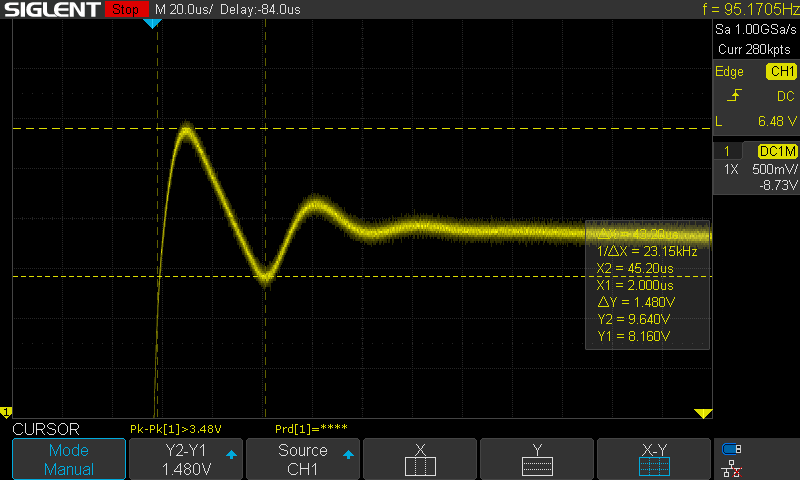
\includegraphics[width=\linewidth]{slike/1.png} 
		\caption{Posnetek zaslona osciloskopa z meritvami časa pozameznega iznihaja}
	\end{figure}

	\subsection*{Analiza rezultatov}
	Za (maksimalno) napetost vsakega pulza lahko zapišemo enačbo 
	\begin{equation}
		U_N = U_0 e^{-\beta ((N-1)t_0 + t_z)}, \footnote{Za $U_1$ zapišemo $U_1 = U_0 e^{-\beta t_z}$}
	\end{equation} ker govorimo o maksimalni napetosti upoštevamo, da je $sin(\omega t) = 1$.
	$\beta$ lahko izrazimo takole
	\begin{equation}
		\begin{split}
			ln(\frac{U_1}{U_N}) = \beta (N-1) t_0 \\
			\beta = \frac{ln(\frac{U_1}{U_N})}{(N-1) t_0}.
		\end{split}
	\end{equation}
	


	\begin{table}[h!]
		\centering
		\begin{tabular}{|c|c|c|c|}
			\hline
			$N$ & $U_n$ [V] & $(N-1)t_0$ [$\mu$ s] & $\beta$ [$10^3 \text{ s}^{-1}$] \\ \hline
			1 & 9,64 & 0 & N/A \\ \hline
			2 & 8,93 & 51,6  & 1,48 \\ \hline
			3 & 8,71 & 92,8  & 1,09 \\ \hline
		\end{tabular}
	\end{table}

	Z aritmetično sredino izračunamo $\overline{\beta} = 1,29 \cdot 10^3 \text{ s}^{-1} \pm 0,2 \cdot 10^3 \text{ s}^{-1}$

\newpage
\section{Gostota zemljinega električnega polja}
	\subsection*{Opis vaje in teoritična podlaga}
	Zemljino magnetno polje deluje na podoben način kot magneti, ki jih poznamo iz vsakdanjega 
	življenja, le da na veliko večjem obsegu. Ko elektroni tečejo skozi žico, ustvarijo 
	magnetno polje okoli nje. Ta pojav je prisoten tudi na atomskem nivoju, kjer elektroni
	krožijo okoli atomov ustvarjajoč majhne tokove in s tem majhna magnetna polja. V
	nekaterih atomih, kot so atomi železa, se ta majhna magentna polja seštevajo in tvorijo
	močnejše magnetno polje. Ta princip je razširljiv vse do obsega Zemlje, kjer gibanje
	tekočega železa v zunanjem jedru, segretem s strani (vročega) notranjega jedra, ustvarja
	konvekcijske tokove. Ti tokovi, skupaj z učinkom Coriolisove sile, ki je posledica
	vrtenja Zemlje, povzročajo, da se tekoče kovinske mase vrtinčijo in ustvarjajo velikansko
	elektromagnetno polje, ki obdaja naš planet. \\

	Kompas nam pokaže smer ''silnic'' \footnote{Kompas se sicer usmeri v smer magnetnega polja,
	magnetna sila deluje pravokotno na smer magetnega polja, za lažjo razlago bom tu napačno
	uporabil izraz silnice, ki sicer pomeni smer delovanja sile} magnetnega polja, to "funkcijo"
	lahko izrabimo za izračun moči magnetnega polja Zemlje. Če s tuljavo ustvarimo magnetno
	polje, ki je pravokotno na zemljino lahko s kompasom določimo, kdaj sta magnetno polje
	Zemlje in tuljave enaka.
	\begin{figure}[h!]
		\centering
		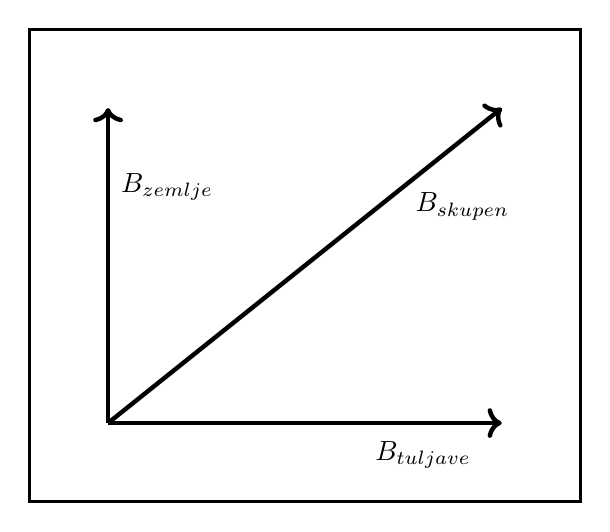
\begin{tikzpicture}
			\draw[black, very thick] (-3,-3) rectangle (4,3);
			\draw[black, ultra thick, ->] (-2, -2) -- (3, -2) node at (2, -2.4) {$B_{tuljave}$};
			\draw[black, ultra thick, ->] (-2, -2) -- (3, 2) node at (2.5, 0.75) {$B_{skupen}$};
			\draw[black, ultra thick, ->] (-2, -2) -- (-2, 2) node at (-1.25, 1) {$B_{zemlje}$};
		\end{tikzpicture}
		\caption{Trikotnik magnetnh polj}
	\end{figure}

	Ker kompas kaže ($\varphi_k$) v smer skupnega magnetnega polja
	($\vec{B_{skupen}} = \vec{B_{zemlje}} + \vec{B_{tuljave}}$), lahko zapišemo
	\begin{equation}
		\tan(\varphi_k) = \frac{B_{tuljave}}{B_{zemlje}} .
	\end{equation}
	Če s tuljavo ustvarimo magnetno polje, ki je po velikosti enako Zemljinemu magnetnemu
	polju, bo $\tan(\varphi_k) = 1 \Rightarrow \varphi_k = \arctan(1) = 45 \text{ °}$.

	\subsection*{Uporabljeni pripomočki}
	Dve tuljavi ($r_{sr} = 7 cm$), kompas, upor ($R = 1 \text{ k}\Omega$), ŠMI z žicami in
	ampermeter
	\subsection*{Tabela meritev}
	\begin{table}[h!]
		\centering
		\begin{tabular}{|c|c|c|c|c|}
		\hline
		$I$ [mA] & $\varphi$ [°] & $B_{Helm}$ [$\mu$T] & $B_{zeml}$ [$\mu$T] & $\Delta B_{zeml}$ [$\mu$T] \\ \hline
		0,00     & 0,00          & 0,00                   &                        &                               \\ \hline
		1,65     & 25,00         & 19,01                  & 40,76                  & 13,58                         \\ \hline
		2,30     & 30,00         & 26,50                  & 45,89                  & 8,45                          \\ \hline
		3,77     & 42,00         & 43,43                  & 48,23                  & 6,11                          \\ \hline
		5,80     & 53,00         & 66,82                  & 50,35                  & 3,99                          \\ \hline
		7,59     & 58,00         & 87,44                  & 54,64                  & 0,30                          \\ \hline
		8,00     & 60,00         & 92,16                  & 53,21                  & 1,13                          \\ \hline
		9,57     & 62,00         & 110,25                 & 58,62                  & 4,28                          \\ \hline
		19,80    & 70,00         & 228,10                 & 83,02                  & 28,68                         \\ \hline
		\end{tabular}
		\caption{Tabela meritev zemljinega magnetnega polja}
	\end{table}
	\subsection*{Analiza rezultatov}
	Ker smo uporabili Helmholtzovo tuljavo, bomo $B_{tuljave}$ označili z $B_{Helm}$, ker 
	poznamo dolžino tuljave in število ovojev, lahko izračunamo magnento polje, ki jo ustvari
	\begin{equation}
		B = \mu_0 \frac{NI}{l}.
	\end{equation}

	Izračunana vrednot magnetnega polja Zemlje je $B = 54,3 \cdot 10^-6 \text{ T} (1 \pm 0,09)$,
	kar je le 12 \% več od vrednosti, ki sem jo našel na internetu \cite{noaa} ($B = 48,3 \text{ } \mu \text{T} $)
	\footnote{Vrednost za Ljubljano, 15. 11. 2023}

\newpage
\section{Merjenje goriščne razdalje leč}
	\subsection*{Opis vaje in teoritična podlaga}
	Vaja zajema merjenje goriščne razdalje konveksne (zbiralne), konkavne (razpršilne) in 
	stavljene leče. Formula za izračun goriščne razdalje leče je $f = 2R$, kjer je $f$ 
	goriščna razdalja, $R$ pa polmer leče ali zrcala. Goriščna razdalja sestavljene leče
	(dve zaporedni leči) se izračuna z $\frac{1}{f} = \frac{1}{f_1} + \frac{1}{f_2} - \frac{d}{f_1 \cdot f_2}$
	\cite{lece}, kjer sta $f_1$ in $f_2$ goriščni razdalji sestavnih leč, $d$ pa razdalja med njima.

	\subsection*{Uporabljeni pripomočki}
	Svetilka v ohišju z režami, ŠMI z žicami, milimeterski papir, svinčnik, geotrikotnik, 
	konveksna in konkavna leča ($R = 35 \text{ mm}$ za obe leči)
	\subsection*{Skice}
	
	%Zbiralna leča
	\begin{figure}[h!]
		\centering
		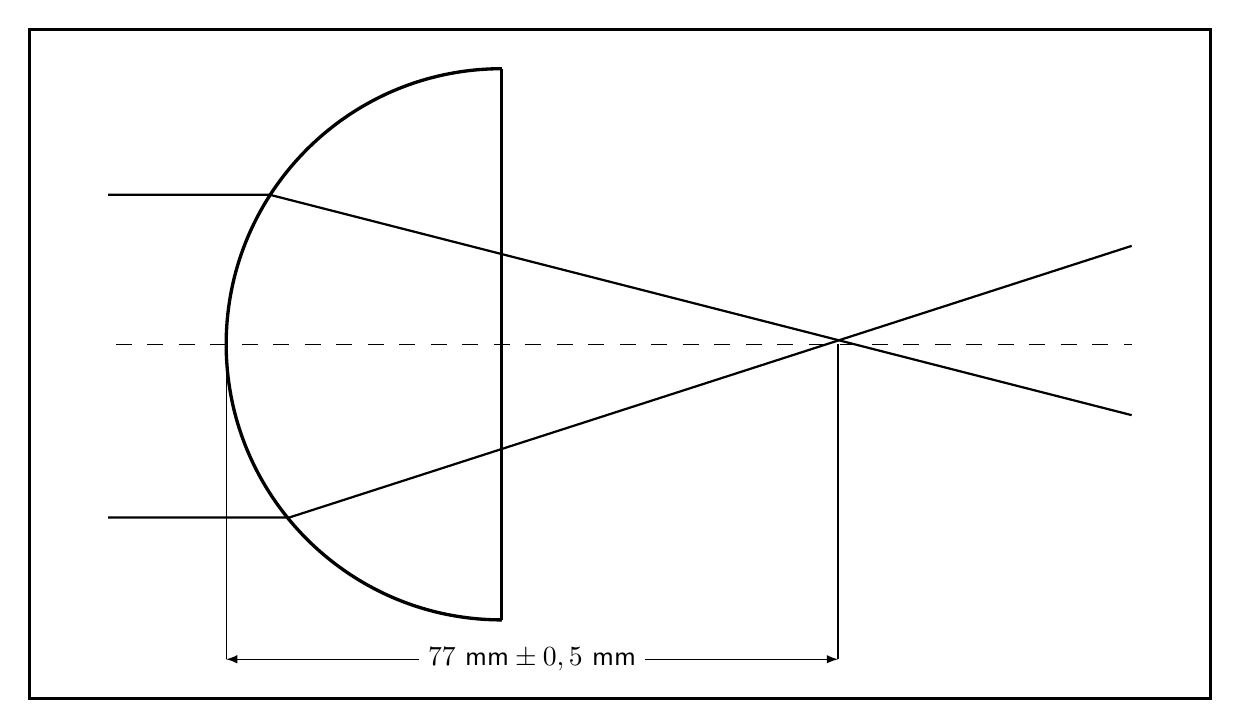
\begin{tikzpicture}
			\draw[black, very thick] (-6,-4.5) rectangle (9,4);
			\draw[dash=on 2mm off 2mm phase -1mm] (-5, 0) -- (8, 0);
				
			%leča
			\draw[very thick] (0, 3.5) arc (90:270:3.5);
			\draw[very thick] (0, 3.5) -- (0, -3.5);
			
			%žarki
			\draw[thick] (-5, 1.9) -- (-2.95, 1.9) -- (8, -0.9);
			\draw[thick] (-5, -2.2) -- (-2.7, -2.2) -- (8, 1.25);
			
			%meritev
			\draw (-3.5, 0) -- (-3.5, -4);
			\draw (4.27, 0) -- (4.27, -4);
			\draw[dimen] (-3.5, -4) -- (4.27, -4) node {$77 \text{ mm} \pm 0,5 \text{ mm}$};
		\end{tikzpicture}
		\caption{Zbiralna leča}
	\end{figure}
	
	%Razpršilna leča
	\begin{figure}[h!]
		\centering
		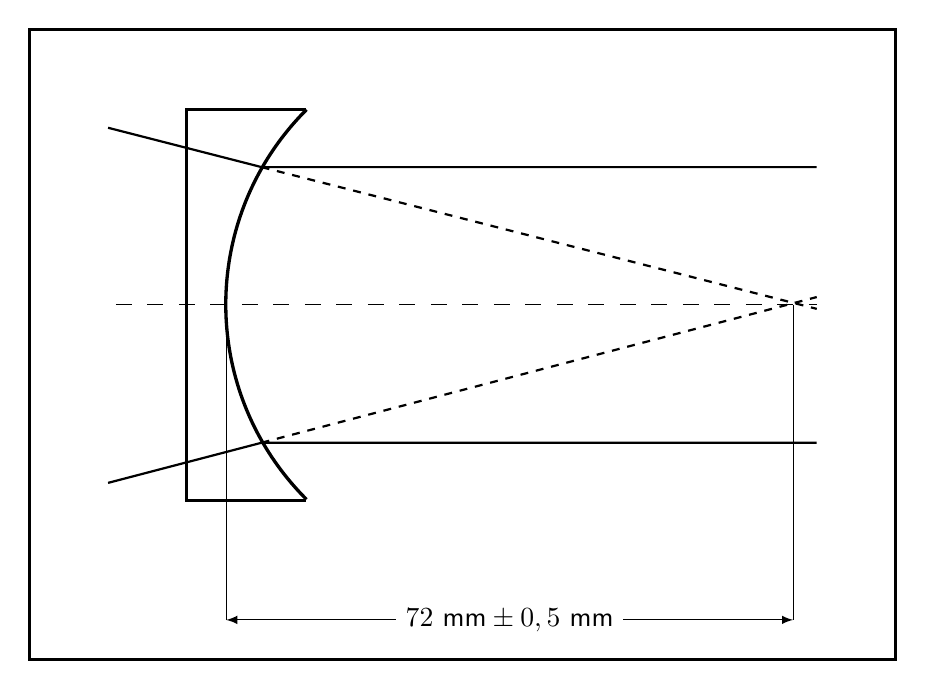
\begin{tikzpicture}
			\draw[black, very thick] (-6,-4.5) rectangle (5, 3.5);
			\draw[dash=on 2mm off 2mm phase -1mm] (-5, 0) -- (4, 0);
			
			%leča
			\draw[very thick] (-2.48, 2.48) arc (135:225:3.5);
			\draw[very thick] (-2.48, 2.48) -- (-4, 2.48) -- (-4, -2.48) -- (-2.48, -2.48);
			
			%žarki
			\draw[thick] (4, 1.75) -- (-3.05, 1.75) -- (-5, 2.25);
			\draw[thick] (4, -1.75) -- (-3.05, -1.75) -- (-5, -2.26);
			\draw[thick, dash=on 1mm off 1mm phase 0mm] (-3.05, 1.75) -- (4, -0.05);
			\draw[thick, dash=on 1mm off 1mm phase 0mm] (-3.05, -1.75) -- (4, 0.1);
			
			%meritev
			\draw (-3.5, 0) -- (-3.5, -4);
			\draw (3.7, 0) -- (3.7, -4);
			\draw[dimen] (-3.5, -4) -- (3.7, -4) node {$72 \text{ mm} \pm 0,5 \text{ mm}$};
		\end{tikzpicture}
		\caption{Razpršilna leča}
	\end{figure}
	
	%Sestavljena leča
	\begin{figure}[h!]
		\makebox[\textwidth][c]{
			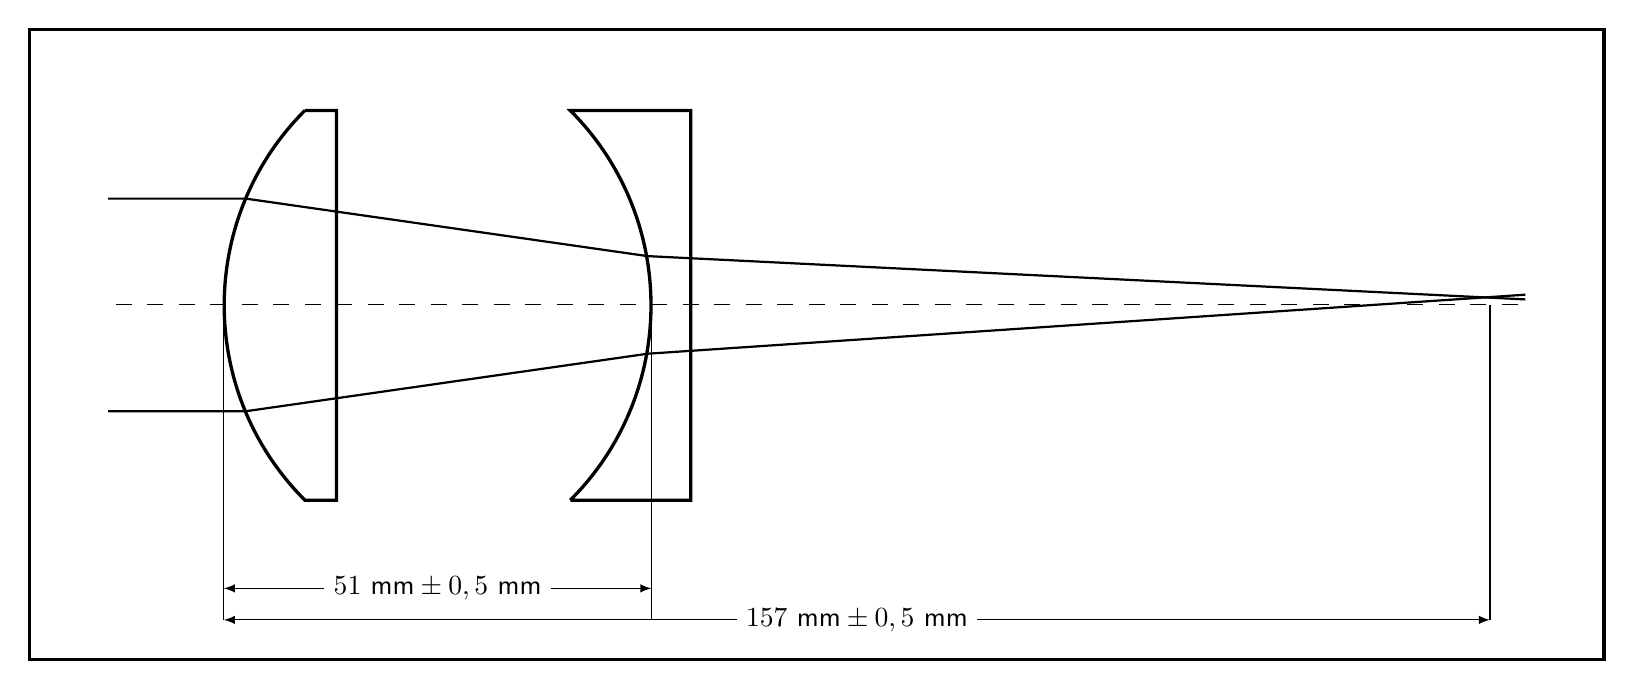
\begin{tikzpicture}
				\draw[black, very thick] (-10,-4.5) rectangle (10, 3.5);
				\draw[dash=on 2mm off 2mm phase -1mm] (-9, 0) -- (9, 0);
				
				%zibralna leča
				\draw[very thick] (-6.5, 2.47) arc (135:225:3.5) -- (-6.1, -2.48) -- (-6.1, 2.47) -- (-6.5, 2.47);
				
				%razpršilna leča
				\draw[very thick] (-3.13, -2.48) arc (-45:45:3.5) -- (-1.6, 2.47) -- (-1.6, -2.48) -- (-3.13, -2.48);
				
				%žarki
				\draw[thick] (-9, 1.35) -- (-7.25, 1.35) -- (-2.15, 0.62) -- (9, 0.07);
				\draw[thick] (-9, -1.35) -- (-7.25, -1.35) -- (-2.15, -0.62) -- (9, 0.13);
				
				%meritve
				\draw (-7.53, 0) -- (-7.53, -4);
				\draw (8.55, 0) -- (8.55, -4);
				\draw[dimen] (-7.53, -4) -- (8.55, -4) node {$157 \text{ mm} \pm 0,5 \text{ mm}$};
				\draw (-2.1, 0) -- (-2.1, -4);
				\draw[dimen] (-7.53, -3.6) -- (-2.1, -3.6) node {$51 \text{ mm} \pm 0,5 \text{ mm}$};
			\end{tikzpicture}
			}
		\caption{Sestavljena leča}
	\end{figure}
	\newpage
	\subsection*{Analiza rezultatov}
	Izmerjena goriščna razdalja konveksne leče je $f = 77 \text{ mm} \pm 0,5 \text{ mm}$,
	izračunana razdalja pa je 
	\begin{equation}
		f = 2R = 2 \cdot 35 \text{ mm} = 70 \text{ mm}
	\end{equation}.\\
	Za konkavno lečo pa sem izmeril goriščno razdaljo $f = 72 \text{ mm} \pm 0,5 \text{ mm}$, 
	izračunana goriščna razdalja je 
	\begin{equation}
		f = -2R = -2 \cdot 35 \text{ mm} = -70 \text{ mm}
	\end{equation}.\\
	Pri sestavljeni lečo sem izmeril goriščno razdaljo $f = 157 \text{ mm} \pm 0,5 \text{ mm}$,
	izračunal pa sem
	\begin{equation}
		\begin{split}
			\frac{1}{f} &= \frac{1}{f_1} + \frac{1}{f_2} - \frac{d}{f_1 \cdot f_2} \\
			f &= (\frac{1}{-70 \text{ mm}} + \frac{1}{70 \text{ mm}} - \frac{51 \text{ mm}}{-70 \text{ mm} \cdot 70 \text{ mm}})^{-1}\\
			f &= 102 \text{ mm}
		\end{split}
	\end{equation}
	če za izračun uporabimo izmerjene vrednosti dobimo, da je goriščna razdalja $f = 120 \text{ mm}$.
	Kljub vsemu osnovne formule za izračun goriščne razdalje sestavljene leče sam ne morem
	potrditi.


\newpage
\section{Plinski emisijski spektri}
	\subsection*{Opis vaje in teoritična podlaga}
	Elektroni lahko prehajajo med večimi energijskimi nivoji. Zaradi potrebe po ohranitvi
	energije, se pri prehajanu iz višjega eregijskega nivoji na nižji nivo sprosti preostanek
	energije v obliki fotona. Valovna dolžina je odvisna od energije fotona po enačbi $f = \frac{E_f}{h}$,
	kjer je $h = 6,62607015 \cdot 10^{-34} \frac{\text{J}}{\text{Hz}}$ oz. Planck-ova konstanta.
	Vredno je povdariti, da to ni nek približek, Placnk-ova konstanta ima tako
	kot svetloba hitrost točno vrednost.
	\begin{quote} 
		The kilogram, symbol kg, is the SI unit of mass. It is defined by taking the fixed
		numerical value of the Planck constant $h$ to be $6,62607015 \cdot 10^{-34}$ when
		expressed in the unit $\text{J} \cdot \text{s}$, which is equal to $\text{kg} \cdot \text{m}^2 \cdot \text{s}^{-1}$,
		where the metre and the second are defined in terms of c and $\Delta \nu \text{C}$. \cite{redef}
	\end{quote}

	Kot je to vidno na fotografiji \ref{fig:mavrica} lahko z uklonsko mrežico svetlomo razvrstimo
	po njeni valnovni dolžini, ker so v emisijskem spektru prisotne le nekatere valovne dolžine,
	vidimo samo tiste, ki jih atom lahko oddaja.

	\begin{figure}[h!]
		\centering
		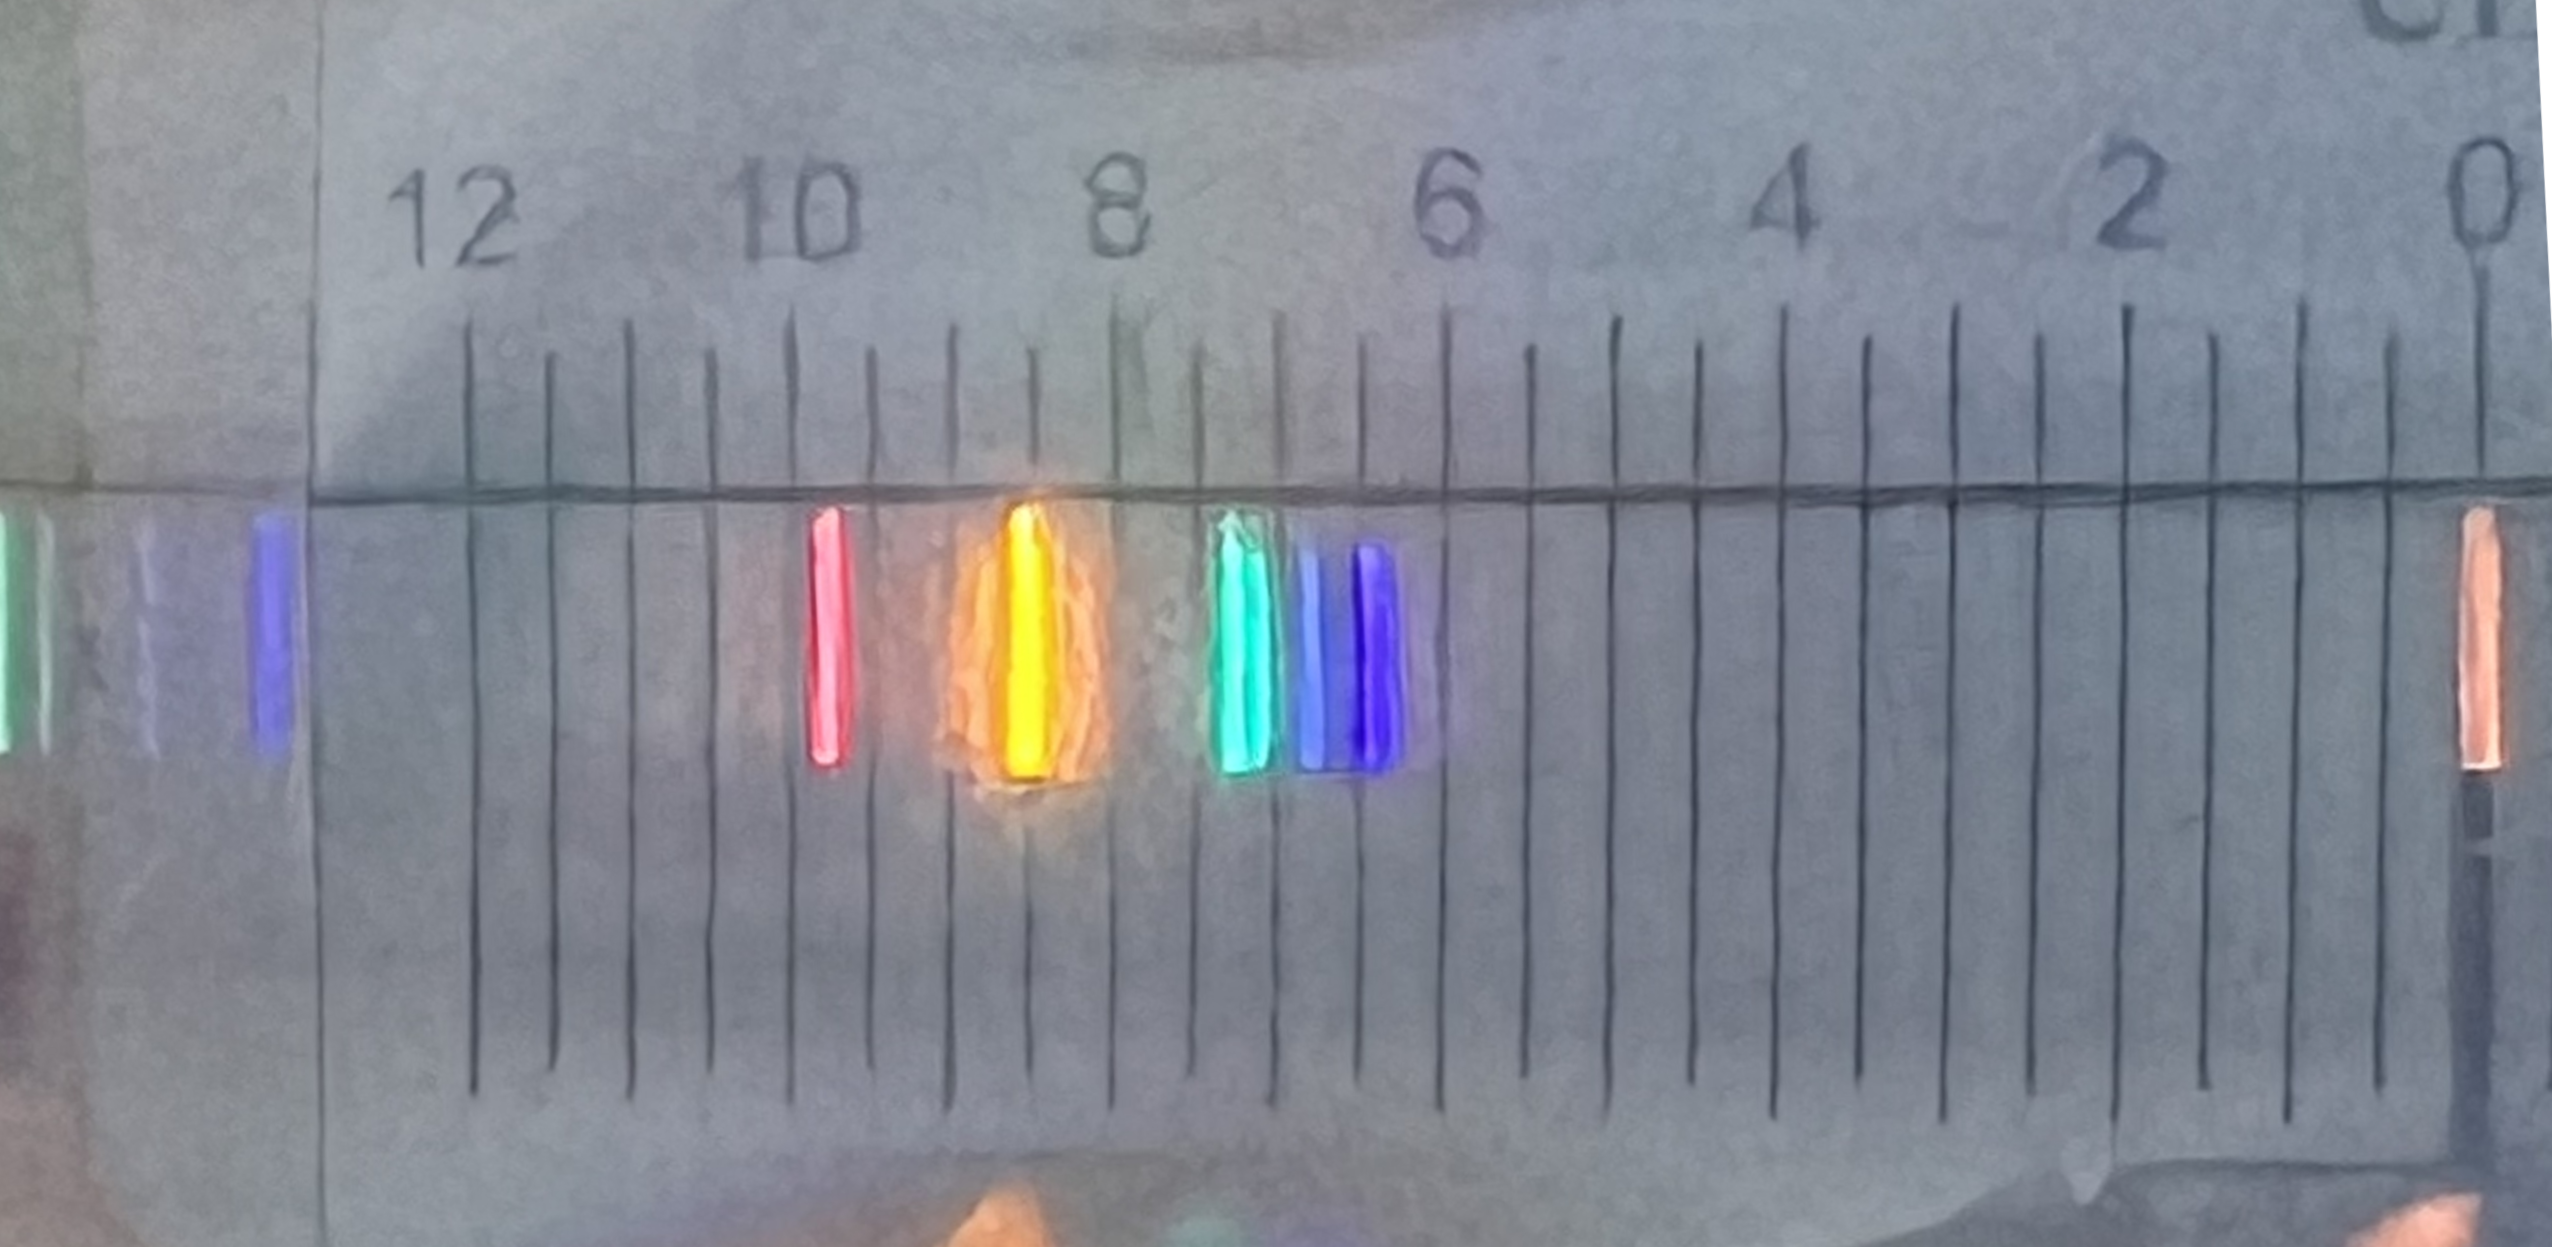
\includegraphics[width=0.8\linewidth]{slike/IMG_3563.png}
		\caption{Emisijski spekter helija}
		\label{fig:mavrica}
	\end{figure}

	Uklonski kot fotonov določene valovne dolžile lahko izračunamo z
	\begin{equation}
		\lambda = \frac{d \sin{\beta}}{N}
	\end{equation}
	kot $\beta$ pa lahko izračunamo z
	\begin{equation}
		\beta=\arctan{\frac{a}{l}}
	\end{equation}.

	Ko združomo obe enačbi, in upoštevamo, da je $N = 1$, saj je dobro viden le prvi red odmikov,
	$d = 300 \frac{1}{\text{mm}}$ in $l = 40 \text{ cm}$ dobimo enačbo za izračun valovne dolžine:
	\begin{equation}
		\lambda = 3 * 10^{-6} \text{ m} \cdot \sin{(\arctan{(\frac{a}{40 \text{ cm}})})}
	\end{equation}

	\null
	\subsection*{Uporabljeni pripomočki}
	Spektralne cevi različnih plinov v ohišju z napetostnim virom, uklonska mrežica s 300 črtami/mm
	\subsection*{Meritve}
	\subsubsection*{Argon}
	\begin{table}[h!]
		\centering
		\begin{tabular}{|c|c|c|c|c|c|c|c|}
			\hline
			barva 		& $a_l$ [cm]	& $a_d$ [cm]	& $a$ [cm]	& $\beta$ [°]	& $\lambda_{izmerjena}$ [nm]	& $\lambda_{prava}$ [nm]		\\ \hline
			vijolična	& 6,30 			& 6,30 			& 6,30		& 8,95			& 466,75						& 462,54 \cite{specters-nist}	\\ \hline
			zelena		& 8,30 			& 8,30 			& 8,30		& 11,72			& 609,52						& 613,38 \cite{specters-nist}	\\ \hline
			roza		& 8,80 			& 8,80 			& 8,80		& 12,41			& 644,59						& 643,51 \cite{specters-nist}	\\ \hline
		\end{tabular}
	\end{table}

	\subsubsection*{Helij}
	\begin{table}[h!]
		\centering
		\begin{tabular}{|c|c|c|c|c|c|c|c|}
			\hline
			barva		& $a_l$ [cm]	& $a_d$ [cm]	& $a$ [cm]	& $\beta$ [°]	& $\lambda_{izmerjena}$ [nm]	& $\lambda_{prava}$ [nm]		\\ \hline
			vijolična	& 6,40			& / 			& 6,40		&  9,09			& 473,97						& 471,32 \cite{specters-nist}	\\ \hline
			modra		& 6,80			& / 			& 6,80		&  9,65			& 502,79						& 501,57 \cite{specters-nist}	\\ \hline
			cyan		& 7,30			& / 			& 7,30		& 10,34			& 538,60						& 587,56 \cite{specters-nist}	\\ \hline
			oranžna		& 8,60			& / 			& 8,60		& 12,13			& 630,59						& 667,82 \cite{specters-nist}	\\ \hline
			rdeča		& 9,70			& /				& 9,70		& 13,63			& 707,01						& 706,52 \cite{specters-nist}	\\ \hline
		\end{tabular}
	\end{table}

	\null
	\subsection*{Analiza rezultatov}
	Meritve so presenetljivo točne, saj je povprečno relativno odstopanje od pravih vrednosti
	največ 8 \%, povprečno pa 1,5 \%. 



\newpage
\begingroup
\makeatletter
	\section{Viri in literatura}
	\nocite{*}
	\printbibliography[heading=none]
\makeatother
\endgroup
\newpage

\begin{samepage}
	\thispagestyle{empty}
	\section*{Izjava o avtorstvu}
	Izjavljam, da so poročila v celoti moje avtorsko delo, ki sem ga 
	izdelal samostojno s pomočjo navedene literature in pod vodstvom mentorja.

	\vfill
	
	\today \hfill Jaka Kovač
	
	\vspace{3 cm}
\end{samepage}

\end{document}
